\documentclass{article}
\usepackage[utf8]{inputenc}

\usepackage{tabularx, booktabs}

% This package allows for automatic conversion of eps figures to pdf
\usepackage{graphics}
\usepackage{epstopdf} 
\graphicspath{ {.}{04/} }
%\DeclareGraphicsExtensions{.pdf,.eps,.png}



\usepackage{amsmath, amssymb}
\usepackage[margin=1in]{geometry}
\usepackage{graphicx}
\usepackage{xcolor}

% To set the enumeration method
\usepackage[shortlabels]{enumitem}

\usepackage[T1]{fontenc}
\usepackage[utf8]{inputenc}
\usepackage{lmodern}

\title{PM511 b: Group 7 Homework Assignment 4}
\author{Group 7}
\date{Due: Feb 29, 2019}

\begin{document}

% We use this command to change the font of the entire document. We can take it out if you want :)
\fontfamily{lmss}\selectfont

\maketitle

\section{Question 1}
 Evaluate the association between the dependent variable of high systolic blood pressure (cut at 140 mmHg) and independent variables of age (as a continuous variable; center the age variable at age 60) and overweight.
 
 \textit{Preamble:} Before working on the solution, we need to load the data and generate the variables that we will be using. The code to do so follows:
 
 \begin{verbatim}
clear all
set more off
set trace off

use vitals, clear
global outregopts tex(fragment) label dec(3)

// Previous variables created
gen hibp = sbp > 140 if sbp != .
gen bmi = 703 * weight / height^2 if (weight != . & sbp != .)
gen overweight = bmi >= 25 if bmi != .

lab var hibp "High Blood Pressure (yes/no)"
lab var overw "Overweight (yes/no)"
lab var age "Age (years)"

egen     age_mean = mean(age)
gen age_cent = age-age_mean
lab var age_cent "Age (mean centered)"

gen age_cent60 = age - 60
lab var age_cent60 "Age centered at 60"
\end{verbatim}

Also, we wrote a Stata program to compute predicted probabilities that we use later:

\begin{verbatim}
// Program to predict disease for individuals with 0 or 5 in s
prog def predictedprobs
    preserve
    quietly {
        drop _all
        set obs 2
        gen age_cent60 = 70*(_n == 1) + 50*(_n == 2) - 60
        gen overweight = _n == 1
        predict pred_prob
        noi list
    }
    restore
end
\end{verbatim}
 
 \begin{enumerate}[a.]
     \item  Evaluate each independent variable (age and overweight) in a separate model.
     
     \textit{Solution} We use the stata module outreg2 to save the regression results. The code and output follows:
     
\begin{verbatim}
. glm hibp age_cent60, link(logit) family(binomial)

Iteration 0:   log likelihood = -1049.7143  
Iteration 1:   log likelihood = -1042.5151  
Iteration 2:   log likelihood = -1042.4814  
Iteration 3:   log likelihood = -1042.4814  

Generalized linear models                          No. of obs      =      2326
Optimization     : ML                              Residual df     =      2324
                                                   Scale parameter =         1
Deviance         =  2084.962726                    (1/df) Deviance =   .897144
Pearson          =  2293.666101                    (1/df) Pearson  =  .9869475

Variance function: V(u) = u*(1-u)                  [Bernoulli]
Link function    : g(u) = ln(u/(1-u))              [Logit]

                                                   AIC             =  .8980923
Log likelihood   = -1042.481363                    BIC             = -15930.47

------------------------------------------------------------------------------
             |                 OIM
        hibp |      Coef.   Std. Err.      z    P>|z|     [95% Conf. Interval]
-------------+----------------------------------------------------------------
  age_cent60 |   .0828624   .0063965    12.95   0.000     .0703256    .0953993
       _cons |  -1.509351   .0574642   -26.27   0.000    -1.621978   -1.396723
------------------------------------------------------------------------------

. outreg2 using part1.tex, replace stats(coef se ci tstat) $outregopts
part1.tex
dir : seeout

. 
. glm hibp overweight, link(logit) family(binomial)

Iteration 0:   log likelihood = -1129.2768  
Iteration 1:   log likelihood = -1128.0478  
Iteration 2:   log likelihood =  -1128.047  
Iteration 3:   log likelihood =  -1128.047  

Generalized linear models                          No. of obs      =      2325
Optimization     : ML                              Residual df     =      2323
                                                   Scale parameter =         1
Deviance         =  2256.093964                    (1/df) Deviance =  .9711984
Pearson          =         2325                    (1/df) Pearson  =  1.000861

Variance function: V(u) = u*(1-u)                  [Bernoulli]
Link function    : g(u) = ln(u/(1-u))              [Logit]

                                                   AIC             =  .9720834
Log likelihood   = -1128.046982                    BIC             = -15750.58

------------------------------------------------------------------------------
             |                 OIM
        hibp |      Coef.   Std. Err.      z    P>|z|     [95% Conf. Interval]
-------------+----------------------------------------------------------------
  overweight |   .5005193   .1246392     4.02   0.000      .256231    .7448076
       _cons |  -1.805273   .1090043   -16.56   0.000    -2.018918   -1.591629
------------------------------------------------------------------------------

. outreg2 using part1.tex, append stats(coef se ci tstat) $outregopts
part1.tex
dir : seeout
\end{verbatim}
     
     \item  Evaluate the two independent variables in the same model.
     
     \textit{Solution} The code and output follows:
     
\begin{verbatim}
. glm hibp age_cent60 overweight, link(logit) family(binomial)

Iteration 0:   log likelihood =  -1037.362  
Iteration 1:   log likelihood = -1027.7196  
Iteration 2:   log likelihood = -1027.6845  
Iteration 3:   log likelihood = -1027.6845  

Generalized linear models                          No. of obs      =      2325
Optimization     : ML                              Residual df     =      2322
                                                   Scale parameter =         1
Deviance         =   2055.36908                    (1/df) Deviance =  .8851719
Pearson          =  2267.806966                    (1/df) Pearson  =  .9766611

Variance function: V(u) = u*(1-u)                  [Bernoulli]
Link function    : g(u) = ln(u/(1-u))              [Logit]

                                                   AIC             =  .8866104
Log likelihood   =  -1027.68454                    BIC             = -15943.56

------------------------------------------------------------------------------
             |                 OIM
        hibp |      Coef.   Std. Err.      z    P>|z|     [95% Conf. Interval]
-------------+----------------------------------------------------------------
  age_cent60 |    .086753   .0065229    13.30   0.000     .0739683    .0995376
  overweight |   .6875901   .1319508     5.21   0.000     .4289712     .946209
       _cons |  -2.019406   .1183531   -17.06   0.000    -2.251373   -1.787438
------------------------------------------------------------------------------

. outreg2 using part1.tex, append stats(coef se ci tstat) $outregopts
part1.tex
dir : seeout
\end{verbatim}
     
     \item  Create a table of results that reports the unadjusted and mutually adjusted parameter estimates, along with 95$\%$ confidence intervals.  
     
     Is there any evidence to suggest that the association of overweight with high blood pressure is confounded by age?  Explain your answer.
     
     \textit{Solution}: For this section, we just used the table generated by outreg2:
     
     \begin{tabular}{l*{3}{m{.2\linewidth}}} \hline
 & (1) & (2) & (3) \\
VARIABLES & High Blood Pressure (yes/no) & High Blood Pressure (yes/no) & High Blood Pressure (yes/no) \\ \hline
Age centered at 60 & 0.083*** &  & 0.087*** \\
 & (0.006) &  & (0.007) \\
 & 0.070 - 0.095 &  & 0.074 - 0.100 \\
 & (12.954) &  & (13.300) \\
Overweight (yes/no) &  & 0.501*** & 0.688*** \\
 &  & (0.125) & (0.132) \\
 &  & 0.256 - 0.745 & 0.429 - 0.946 \\
 &  & (4.016) & (5.211) \\
Constant & -1.509*** & -1.805*** & -2.019*** \\
 & (0.057) & (0.109) & (0.118) \\
 & -1.622 - -1.397 & -2.019 - -1.592 & -2.251 - -1.787 \\
 & (-26.266) & (-16.561) & (-17.063) \\
 &  &  &  \\
 Observations & 2,326 & 2,325 & 2,325 \\ \hline
\multicolumn{4}{c}{Below each estimate we have: Standard Errors, 95\% Confidence Interval, and t-statistic.} \\
\multicolumn{4}{c}{ *** p$<$0.01, ** p$<$0.05, * p$<$0.1} \\
\end{tabular}

     
     The coefficient for Overweight changes from 0.501 (in the model excluding age), to 0.688 (in the model including age), representing a change of about 37\% increment with respect to the baseline model, hence we can say that overweight is confounded by age.
     
     \item Write a short paragraph interpreting your parameter estimates and providing a basic conclusion regarding the association of high blood pressure with age and overweight.
     
     \textit{Solution}: Both variables, overweight and age, are significant predictors of High Blood Pressure (HBP) at 99\%, regardless of whether we model jointly in a single model or separately in two different models, this is, the significance of the effects is robust to the two specifications. In particular, at the 95\% confidence, looking at the model that includes both variables as linear predictors of HBP, Overweight has a positive effect size that lies in the interval [0.429, 0.946], while age (centered at 60) has an effect magnitude within [0.074, 0.100], both with p-values < 0.01. It is important to notice that Age is a confounder of Overweight. 
     
     \item Using the fitted two-variable model (age and overweight), calculate the logit and the predicted probability of high blood pressure among: a person aged 70 who is overweight. A person aged 50 who is not overweight.
     
     \textit{Solution}: Using the function generated in at the beginning:
     
\begin{verbatim}
. predictedprobs

     +--------------------------------+
     | age_c~60   overwe~t   pred_p~b |
     |--------------------------------|
  1. |       10          1   .3859696 |
  2. |      -10          0   .0528032 |
     +--------------------------------+

\end{verbatim}

Where the first column is age centered at 60, hence row 1 is of a 70 years old individual with overweight, and the second one is a 50 years old person with no overweight.
     
 \end{enumerate}


\section{Question 2} 
  Explore the relationship between high blood pressure and age more carefully.  Specifically, is the relationship linear on the logit scale?  Evaluate the relationship using:
\begin{enumerate}[a.]
    \item  Grouped smooth with quartiles 
    
    \textit{Solution}: Stata code
    
\begin{verbatim}
sort age
egen age_quant = cut(age), group(4) lab
lab var age_quant "Age quantile"

logit hibp i.age_quant
mat def betas = e(b)
bysort age: egen age_midpoint = mean(age_quant)
lab var age_mid "Midpoint of the Age quantile"

gen beta = .
forval i = 1/4 {
    replace beta = betas[1, `i'] if age_quant == (`i' - 1)
}
// replace beta = 0 if beta == .
lab var beta "Logit coefficient"

twoway scatter beta age_midpoint || line beta age_midpoint
graph export part2_hibp_vs_age_quant.eps, replace
\end{verbatim}
    
    \begin{figure}[!h]
        \centering
        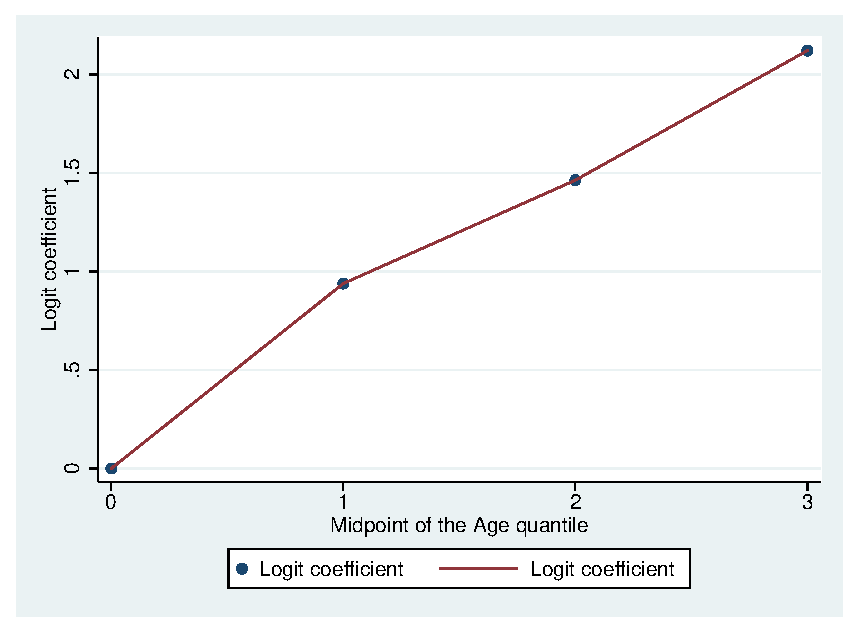
\includegraphics[width=.7\linewidth]{04/part2_hibp_vs_age_quant.eps}
    \end{figure}
    
As we can see, there doesnot appear to be any major issues with linearity on the logit scale.
    
    \item Lowess smoothing
    
    \textit{Solution}: Stata code:
    
\begin{verbatim}
lowess hibp age, addplot(scatter hibp age) legend(off) logit
graph export part2_hibp_vs_age_lowess.eps, replace
\end{verbatim}
    
    \begin{figure}{!h}
        \centering
        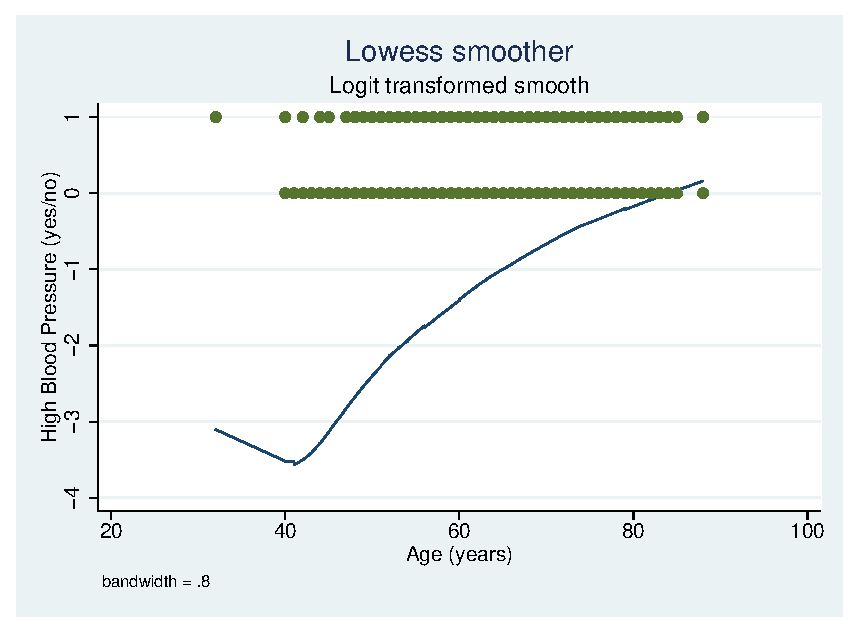
\includegraphics[width=.7\linewidth]{04/part2_hibp_vs_age_lowess.eps}
    \end{figure}
    
Thus, although there appears to be some issues with linearity in the lower extreme observations due to a possible outlier, altogether, there does not appear to be any other remarkable deviations from linearity.
    
    \pagebreak
    
    \item Fractional polynomials.   What is the best one-term and the best two-term model?Are these models better than the linear model (give p-values)? 
    
    The linear term is not significantly different from the 2-term model (p=0.11), neither is the 1-term model (p=0.22).  The linear term is not different from the 1-term model (p=0.084).
     \begin{verbatim}
         fp <AGE>, dimension(2) replace: logit hbp <AGE>
	*the linear term p-value =0.111 does not differ from 2-term
	
	*1-term model.
	fp <AGE>, dimension(1) replace: logit hbp <AGE>
 *the 1-term is -0.5, 8.89+-79.99*(1/sqrt(AGE)), and the linear model is not significantly
 *different p=0.084.
	
	*2-term model
	*4.12 + 64956.65*(1/AGE)^2 + -20787.54*(1/AGE)^2*Ln(AGE)
*the linear model is not different from 2-term, p=0.22


. do "C:\Users\SHANEG~1\AppData\Local\Temp\STDc4_000000.tmp"

. fp <age>, replace: logit hibp <age>
(fitting 44 models)
(....10%....20%....30%....40%....50%....60%....70%....80%....90%...
> .100%)

Fractional polynomial comparisons:
-------------------------------------------------------------------
> -
         age |   df    Deviance   Dev. dif.   P(*)   Powers
-------------+-----------------------------------------------------
> -
     omitted |    0   2273.637    194.694    0.000               
      linear |    1   2084.963      6.020    0.111   1           
       m = 1 |    2   2081.969      3.026    0.220   -.5         
       m = 2 |    4   2078.943      0.000       --   -2 -2       
-------------------------------------------------------------------
> -
(*) P = sig. level of model with m = 2 based on chi^2 of
    dev. dif.

Logistic regression                             Number of obs     =
>       2,326
                                                LR chi2(2)        =
>      194.69
                                                Prob > chi2       =
>      0.0000
Log likelihood = -1039.4716                     Pseudo R2         =
>      0.0856

-------------------------------------------------------------------
> -----------
        hibp |      Coef.   Std. Err.      z    P>|z|     [95% Conf
> . Interval]
-------------+-----------------------------------------------------
> -----------
       age_1 |   64956.65   22327.93     2.91   0.004      21194.7 
>    108718.6
       age_2 |  -20787.54   6305.745    -3.30   0.001    -33146.57 
>   -8428.504
       _cons |   4.118223   .9536049     4.32   0.000     2.249191 
>    5.987254
-------------------------------------------------------------------
> -----------

. fp <age>, dim(1) replace: logit hibp <age>
(fitting 8 models)
(....10%....20%....30%....40%....50%....60%....70%....80%....90%...
> .100%)

Fractional polynomial comparisons:
-------------------------------------------------------------------
> -
         age |   df    Deviance   Dev. dif.   P(*)   Powers
-------------+-----------------------------------------------------
> -
     omitted |    0   2273.637    191.669    0.000               
      linear |    1   2084.963      2.994    0.084   1           
       m = 1 |    2   2081.969      0.000       --   -.5         
-------------------------------------------------------------------
> -
(*) P = sig. level of model with m = 1 based on chi^2 of
    dev. dif.

Logistic regression                             Number of obs     =
>       2,326
                                                LR chi2(1)        =
>      191.67
                                                Prob > chi2       =
>      0.0000
Log likelihood = -1040.9844                     Pseudo R2         =
>      0.0843

-------------------------------------------------------------------
> -----------
        hibp |      Coef.   Std. Err.      z    P>|z|     [95% Conf
> . Interval]
-------------+-----------------------------------------------------
> -----------
       age_1 |  -79.98538   6.354465   -12.59   0.000    -92.43991 
>   -67.53086
       _cons |   8.887089   .8090906    10.98   0.000     7.301301 
>    10.47288
-------------------------------------------------------------------
> -----------

. 
end of do-file


	     \end{verbatim}
    
    \item d: Based on all of your explorations, how would you choose to model the relationship between high blood pressure and age?  Explain your answer, using the information you obtained from each of the 3 approaches (2a-2c). 
    
     The 1-term model has the power =-0.5, and the equation is 8.89-79.99*(1/$\sqrt{AGE}$); the linear model was not statistically significantly different (p=0.084).
     The 2-term model has power -2,-2, and the equation is 4.12+64956.65*($1/AGE)^{2} - 20787.54*(1/AGE)^{2}Ln(AGE)$. Pertinently, according to this test, the linear term was also not statistically significantly different from the 2-term model (p=.111). Moreover, as seen in the prior parts, both the grouped smooth and lowess plots failed to indicate any remarkable departure from linearity on the logit scale. Thus, we will choose the linear model because the models with power terms do not demonstrate a statistically significant difference from the linear model, indicating that they would not offer an improvement, the linearity of the basic linear model on the logit scale is cogently substantiated, and it is most interpret-able.
  \end{enumerate}

\section{Question 3} 
Now use the logistic regression model above to model age in two ways: (1) mean-centered age as a continuous variable; (2) Age categories $(<45, 45-49, 50-54, 55-59, 60-64, 65-69, 70-74, 75-79, and \geq 80). $
Run each age variable in a model with the overweight variable.
\begin{enumerate}[a.]
    \item  Obtain the Wald’s test and likelihood ratio test for age in each model.(Hint: the df for the continuous age = 1; the df for the categorical age variable = 8).
    
    \textit{Solution:} First, we fit the two separate models: one utilizing age (centered at 60 years) as a continuous predictor and one with age as a categorical predictor. The logistic model with age as a continuous predictor was statistically significant ($LR \ \chi^2(2) = 217.84$; $p < .0001$). Moreover, the model utilizing age as a categorical predictor was also statistically significant ($LR \ \chi^2(9) = 219.79$; $p < .0001$).

Pertinently, both models were also found to be statistically significant when compared to the reduced model through a likelihood ratio test and also by the Wald test. For the model with age as a continuous predictor, $LR \ \chi^2(1) = 200.72$ ($p < .0001$) and $Wald \ \chi^2(1) = 176.88$ ($p <.0001$). Thus, the coefficient for centered was statistically significantly different from zero. For the model with age as a categorical predictor, $LR \ \chi^2(8) = 202.67$ ($p < .0001$) and $Wald \ \chi^2(8) = 168.78$ ($p <.0001$). Thus, at least one of the coefficients for the age categories was statistically significantly different from zero. 

\subsubsection*{Stata Code/Output}
\begin{verbatim}
    
. do "C:\Users\SHANEG~1\AppData\Local\Temp\STD3ed4_000000.tmp"

. logit hibp overw

Iteration 0:   log likelihood = -1136.6058  
Iteration 1:   log likelihood = -1128.1189  
Iteration 2:   log likelihood =  -1128.047  
Iteration 3:   log likelihood =  -1128.047  

Logistic regression                             Number of obs     =
>       2,325
                                                LR chi2(1)        =
>       17.12
                                                Prob > chi2       =
>      0.0000
Log likelihood =  -1128.047                     Pseudo R2         =
>      0.0075

-------------------------------------------------------------------
> -----------
        hibp |      Coef.   Std. Err.      z    P>|z|     [95% Conf
> . Interval]
-------------+-----------------------------------------------------
> -----------
  overweight |   .5005193   .1246392     4.02   0.000      .256231 
>    .7448076
       _cons |  -1.805273   .1090043   -16.56   0.000    -2.018918 
>   -1.591629
-------------------------------------------------------------------
> -----------

. est store red

. 
. logit hibp overw age_cent60

Iteration 0:   log likelihood = -1136.6058  
Iteration 1:   log likelihood = -1033.1879  
Iteration 2:   log likelihood = -1027.7016  
Iteration 3:   log likelihood = -1027.6845  
Iteration 4:   log likelihood = -1027.6845  

Logistic regression                             Number of obs     =
>       2,325
                                                LR chi2(2)        =
>      217.84
                                                Prob > chi2       =
>      0.0000
Log likelihood = -1027.6845                     Pseudo R2         =
>      0.0958

-------------------------------------------------------------------
> -----------
        hibp |      Coef.   Std. Err.      z    P>|z|     [95% Conf
> . Interval]
-------------+-----------------------------------------------------
> -----------
  overweight |   .6875901   .1319508     5.21   0.000     .4289712 
>     .946209
  age_cent60 |    .086753   .0065229    13.30   0.000     .0739683 
>    .0995376
       _cons |  -2.019406   .1183531   -17.06   0.000    -2.251373 
>   -1.787438
-------------------------------------------------------------------
> -----------

. lrtest red

Likelihood-ratio test                                 LR chi2(1)  =
>     200.72
(Assumption: red nested in .)                         Prob > chi2 =
>     0.0000

. test age_cent60

 ( 1)  [hibp]age_cent60 = 0

           chi2(  1) =  176.88
         Prob > chi2 =    0.0000

. 
. logit hibp overw i.age_cat

Iteration 0:   log likelihood = -1136.6058  
Iteration 1:   log likelihood = -1036.8862  
Iteration 2:   log likelihood = -1026.8518  
Iteration 3:   log likelihood = -1026.7132  
Iteration 4:   log likelihood = -1026.7128  
Iteration 5:   log likelihood = -1026.7128  

Logistic regression                             Number of obs     =
>       2,325
                                                LR chi2(9)        =
>      219.79
                                                Prob > chi2       =
>      0.0000
Log likelihood = -1026.7128                     Pseudo R2         =
>      0.0967

-------------------------------------------------------------------
> -----------
        hibp |      Coef.   Std. Err.      z    P>|z|     [95% Conf
> . Interval]
-------------+-----------------------------------------------------
> -----------
  overweight |    .645287   .1316101     4.90   0.000     .3873359 
>    .9032382
             |
     age_cat |
       < 50  |   .5843874   .5335077     1.10   0.273    -.4612684 
>    1.630043
       < 55  |   .8863882   .4912535     1.80   0.071     -.076451 
>    1.849227
       < 60  |   1.666156   .4726691     3.52   0.000     .7397415 
>     2.59257
       < 65  |    2.04844   .4697833     4.36   0.000     1.127682 
>    2.969198
       < 70  |   2.385369    .473847     5.03   0.000     1.456646 
>    3.314092
       < 75  |   3.012657   .4803488     6.27   0.000     2.071191 
>    3.954124
       < 80  |   2.776042   .5114615     5.43   0.000     1.773595 
>    3.778488
      >= 80  |   3.365888   .5808775     5.79   0.000     2.227389 
>    4.504387
             |
       _cons |  -3.785872    .469988    -8.06   0.000    -4.707031 
>   -2.864712
-------------------------------------------------------------------
> -----------

. lrtest red

Likelihood-ratio test                                 LR chi2(8)  =
>     202.67
(Assumption: red nested in .)                         Prob > chi2 =
>     0.0000

. test 1.age_cat 2.age_cat 3.age_cat 4.age_cat 5.age_cat ///
> 6.age_cat 7.age_cat 8.age_cat

 ( 1)  [hibp]1.age_cat = 0
 ( 2)  [hibp]2.age_cat = 0
 ( 3)  [hibp]3.age_cat = 0
 ( 4)  [hibp]4.age_cat = 0
 ( 5)  [hibp]5.age_cat = 0
 ( 6)  [hibp]6.age_cat = 0
 ( 7)  [hibp]7.age_cat = 0
 ( 8)  [hibp]8.age_cat = 0

           chi2(  8) =  168.78
         Prob > chi2 =    0.0000

. 
end of do-file

\end{verbatim}


    
    \item  Obtain the Pearson’s and Hosmer-Lemeshow goodness-of-fit statistics for each model and compare.
    
\textit{Solution}: The Pearson $\chi^2$ Goodness and Hosmer-Lemeshow Goodness of Fit statistics for the model with age as a continuous variable were 136.59 ($p = .0014$) and 13.43 ($p=.0978$) respectively. For the model with age as a categorical variable, they were 9.16 ($p=.3287$) and 6.15 ($p=.6307$) respectively. According to these GoF tests, the categorical model seems to provide a better fit; especially since the Pearson's GoF test for age as a continuous predictor was statistically significant. However, recall: age treated continuously might produce issues related to the m-asymptotics. The Hosmer-Lemeshow, after grouping upon deciles of risk, was non-significant, indicating that the model might still be a good fit. Nevertheless, both statistics for the categorical model are lower.

\subsubsection*{Stata Output for GoF Tests:}
\begin{verbatim}

. do "C:\Users\SHANEG~1\AppData\Local\Temp\STD3ed4_000000.tmp"

. 
. quietly logit hibp overw age_cent60

. estat gof

Logistic model for hibp, goodness-of-fit test

       number of observations =      2325
 number of covariate patterns =        94
             Pearson chi2(91) =       136.59
                  Prob > chi2 =         0.0014

. estat gof, group(10) table

Logistic model for hibp, goodness-of-fit test

  (Table collapsed on quantiles of estimated probabilities)
  +--------------------------------------------------------+
  | Group |   Prob | Obs_1 | Exp_1 | Obs_0 | Exp_0 | Total |
  |-------+--------+-------+-------+-------+-------+-------|
  |     1 | 0.0618 |     8 |  10.9 |   225 | 222.1 |   233 |
  |     2 | 0.0853 |     8 |  17.8 |   234 | 224.2 |   242 |
  |     3 | 0.1085 |    24 |  22.9 |   208 | 209.1 |   232 |
  |     4 | 0.1356 |    33 |  29.8 |   205 | 208.2 |   238 |
  |     5 | 0.1581 |    46 |  34.9 |   188 | 199.1 |   234 |
  |-------+--------+-------+-------+-------+-------+-------|
  |     6 | 0.1949 |    46 |  45.1 |   203 | 203.9 |   249 |
  |     7 | 0.2390 |    62 |  56.0 |   192 | 198.0 |   254 |
  |     8 | 0.2895 |    55 |  59.4 |   166 | 161.6 |   221 |
  |     9 | 0.3671 |    59 |  65.1 |   138 | 131.9 |   197 |
  |    10 | 0.7497 |   105 | 104.1 |   120 | 120.9 |   225 |
  +--------------------------------------------------------+

       number of observations =      2325
             number of groups =        10
      Hosmer-Lemeshow chi2(8) =        13.43
                  Prob > chi2 =         0.0978

. estat ic

Akaike's information criterion and Bayesian information criterion

-------------------------------------------------------------------
> ----------
       Model |        Obs  ll(null)  ll(model)      df         AIC 
>        BIC
-------------+-----------------------------------------------------
> ----------
           . |      2,325 -1136.606  -1027.685       3    2061.369 
>   2078.624
-------------------------------------------------------------------
> ----------
               Note: N=Obs used in calculating BIC; see [R] BIC
                     note.

. 
. quietly logit hibp overw i.age_cat

. estat gof

Logistic model for hibp, goodness-of-fit test

       number of observations =      2325
 number of covariate patterns =        18
              Pearson chi2(8) =         9.16
                  Prob > chi2 =         0.3287

. estat gof, group(10) table

Logistic model for hibp, goodness-of-fit test

  (Table collapsed on quantiles of estimated probabilities)
  +--------------------------------------------------------+
  | Group |   Prob | Obs_1 | Exp_1 | Obs_0 | Exp_0 | Total |
  |-------+--------+-------+-------+-------+-------+-------|
  |     1 | 0.0522 |    11 |  14.0 |   310 | 307.0 |   321 |
  |     2 | 0.0720 |    13 |  11.8 |   151 | 152.2 |   164 |
  |     3 | 0.0950 |    28 |  26.2 |   248 | 249.8 |   276 |
  |     4 | 0.1496 |    37 |  35.5 |   238 | 239.5 |   275 |
  |     5 | 0.1863 |    67 |  64.6 |   280 | 282.4 |   347 |
  |-------+--------+-------+-------+-------+-------+-------|
  |     6 | 0.1977 |    25 |  18.6 |    69 |  75.4 |    94 |
  |     7 | 0.2512 |    79 |  82.9 |   251 | 247.1 |   330 |
  |     8 | 0.3158 |    22 |  26.0 |    65 |  61.0 |    87 |
  |     9 | 0.3197 |    62 |  68.4 |   152 | 145.6 |   214 |
  |    10 | 0.5561 |   102 |  98.0 |   115 | 119.0 |   217 |
  +--------------------------------------------------------+

       number of observations =      2325
             number of groups =        10
      Hosmer-Lemeshow chi2(8) =         6.15
                  Prob > chi2 =         0.6307

. estat ic

Akaike's information criterion and Bayesian information criterion

-------------------------------------------------------------------
> ----------
       Model |        Obs  ll(null)  ll(model)      df         AIC 
>        BIC
-------------+-----------------------------------------------------
> ----------
           . |      2,325 -1136.606  -1026.713      10    2073.426 
>    2130.94
-------------------------------------------------------------------
> ----------
               Note: N=Obs used in calculating BIC; see [R] BIC
                     note.

. 
end of do-file

\end{verbatim}

    
    \item   Obtain the AIC and BIC for each model and compare.
    
    \textit{Solution}: The code and output for the AIC and BIC for both models are in the last section's output. For the model with age as a continuous predictor, AIC was 2061.37 and BIC was 2078.62. These values were 2073.43 and 2130.94 respectively for the model with categorical age. Both statistics are lower for the model with age treated as a categorical variable.
    
    \item Which model do you prefer and why?  
    
    \textit{Solution}: We preferred the model with age treated as a continuous variable (and centered at 60). The likelihood ratio test and Wald tests were statistically significant ($p < .0001$ for each respectively) and, although only the Hosmer-Lemeshow GoF test indicated no critical deviation from model assumptions ($p=.0978$), the Pearson's GoF test might have had issues with m-asymptotics. Importantly, both the AIC and BIC for the continuous predictor were less than the AIC and BIC for the categorical one, which is direct evidence that the model utilizing age continuously is a better fit, whereas the GoF tests offer no direct comparison (since they are absolute tests). Furthermore, although age treated categorically might seem to yield more information, the model with centered age has the benefit of being more parsimonious and thus more easily interpret-able. In light of the Hosmer-Lemeshow statistic and the lower AIC and BIC, then, it seemed the better choice.


\begin{table}[!h]
\caption{Logistic Regression Models} 
\begin{center}
\begin{tabular}{lcc} \hline
 & (1) & (2) \\
VARIABLES & High Blood Pressure (yes/no) & High Blood Pressure (yes/no) \\ \hline
 &  &  \\
Age = 1, < 50 years &  & 0.584 \\
 &  & (0.534) \\
 &  & -0.461 - 1.630 \\
 &  & (1.095) \\
Age = 2, < 55 years &  & 0.886* \\
 &  & (0.491) \\
 &  & -0.076 - 1.849 \\
 &  & (1.804) \\
Age = 3, < 60 years &  & 1.666*** \\
 &  & (0.473) \\
 &  & 0.740 - 2.593 \\
 &  & (3.525) \\
Age = 4, < 65 years &  & 2.048*** \\
 &  & (0.470) \\
 &  & 1.128 - 2.969 \\
 &  & (4.360) \\
Age = 5, < 70 years &  & 2.385*** \\
 &  & (0.474) \\
 &  & 1.457 - 3.314 \\
 &  & (5.034) \\
Age = 6, < 75 years &  & 3.013*** \\
 &  & (0.480) \\
 &  & 2.071 - 3.954 \\
 &  & (6.272) \\
Age = 7, < 80 years &  & 2.776*** \\
 &  & (0.511) \\
 &  & 1.774 - 3.778 \\
 &  & (5.428) \\
Age = 8, >= 80 years &  & 3.366*** \\
 &  & (0.581) \\
 &  & 2.227 - 4.504 \\
 &  & (5.794) \\
Overweight (yes/no) & 0.688*** & 0.645*** \\
 & (0.132) & (0.132) \\
 & 0.429 - 0.946 & 0.387 - 0.903 \\
 & (5.211) & (4.903) \\
Age (Centered at 60) & 0.087*** &  \\
 & (0.007) &  \\
 & 0.074 - 0.100 &  \\
 & (13.300) &  \\
Constant & -2.019*** & -3.786*** \\
 & (0.118) & (0.470) \\
 & -2.251 - -1.787 & -4.707 - -2.865 \\
 & (-17.063) & (-8.055) \\
 &  &  \\
Observations & 2,325 & 2,325 \\
Pearson-Chi2 & 136.59 & 9.16 \\
Hosmer-Lemeshow-Chi2 & 13.43 & 6.15 \\
AIC & 2061.37 & 2073.43 \\
 BIC & 2078.62 & 2130.94 \\ \hline
\multicolumn{3}{c}{Below each estimate we have: Standard Errors, 95\% Confidence Interval, and t-statistic.} \\
\multicolumn{3}{c}{ *** p$<$0.01, ** p$<$0.05, * p$<$0.1} \\
\end{tabular}
\end{center}
\end{table}
\clearpage

\subsection*{Stata Code:}
\begin{verbatim}
    clear all
set more off
set trace off

cd "C:\Users\Shane Guglielmo\Desktop\PM511b\HW4"

use vitals, clear
global outregopts tex(fragment) label dec(3)

// Previous variables created
gen hibp = sbp > 140 if sbp != .
gen bmi = 703 * weight / height^2 if (weight != . & sbp != .)
gen overweight = bmi >= 25 if bmi != .

lab var hibp "High Blood Pressure (yes/no)"
lab var overw "Overweight (yes/no)"
lab var age "Age (years)"

egen     age_mean = mean(age)
gen age_cent = age-age_mean
lab var age_cent "Age (mean centered)"

gen age_cent60 = age - 60
lab var age_cent60 "Age centered at 60"


gen age_cat = 0 + ///
    (age >= 45) + ///
    (age >= 50) + ///
    (age >= 55) + ///
    (age >= 60) + ///
    (age >= 65) + ///
    (age >= 70) + ///
    (age >= 75) + ///
    (age >= 80) if age != .


local labs = `"lab def agecatlab 0 "< 45""'
forval i = 1/7 {
    local labs = `"`labs' `i' "< `=`i'*5 + 45'""'
}
local labs = `"`labs' 8 ">= 80""'

`labs'
lab values age_cat agecatlab 

// Checking proper labeling
tabstat age, by(age_cat) s(min max)

// Program to get the stats
cap program drop goftest
prog def goftest, rclass
    // GOF commands
    estat gof
    return local gofpearson : di round(r(chi2), 0.01)
    estat gof, group(10) table
    return local gofhosmer : di round(r(chi2), 0.01)
    
    // AIC
    estimates stats
    tempname mat1 AIC BIC
    mat def `mat1' = r(S)
    mat def `AIC' = `mat1'[1, "AIC"]
    mat def `BIC' = `mat1'[1, "BIC"]
    return local aic : di round(`=`AIC'[1,1]', 0.01)
    return local bic : di round(`=`BIC'[1,1]', 0.01)
end

logit hibp age_cent60 overw
goftest
outreg2 using part3.tex, replace stats(coef se ci tstat) $outregopts ///
    addtext( ///
        Pearson-Chi2, `=r(gofpearson)', ///
        Hosmer-Lemeshow-Chi2, `=r(gofhosmer)', ///
        AIC, `=r(aic)', ///
        BIC, `=r(bic)' ///
    )

logit hibp i.age_cat overw
goftest
outreg2 using part3.tex, append stats(coef se ci tstat) $outregopts ///
    addtext( ///
        Pearson-Chi2, `=r(gofpearson)', ///
        Hosmer-Lemeshow-Chi2, `=r(gofhosmer)', ///
        AIC, `=r(aic)', ///
        BIC, `=r(bic)' ///
    )
\end{verbatim}

    
\end{enumerate}

\section{Question 4}
 For your preferred model above, plot the diagnostic statistics and interpret. 
 
  \begin{enumerate}
    \item Are there any problematic observations?
    
    \textit{Solution}: From figures and tables, we can see there are 6 covariates patterns of 153 patients had delta chi square larger than 4, which include 1 pattern 1 patient larger than 40. If deleting these patients would decrease the Pearson $\chi^2$ Goodness of Fit. \par
    A total of 7 covariates patterns of 127 patients had delta deviance larger than 4. Deleting these patients would have higher change in the deviance residuals. \par
    All patients delta beta were below 0.3, which indicates deleting any observations with same covariate pattern are not likely to change much of the coefficients. \par
    From Delta $\chi^2$ predicted probability proportional to delta beta figure, a few patterns with high probability change of beta had delta chi-square above 4. \par
    In general, consider there are a few covariates pattern that maybe problematic and need further exploration.
    
    % This is equivalent to make macros in latex
    \def\figwidths{.8\linewidth}
    
    
    \begin{figure}
    \centering
    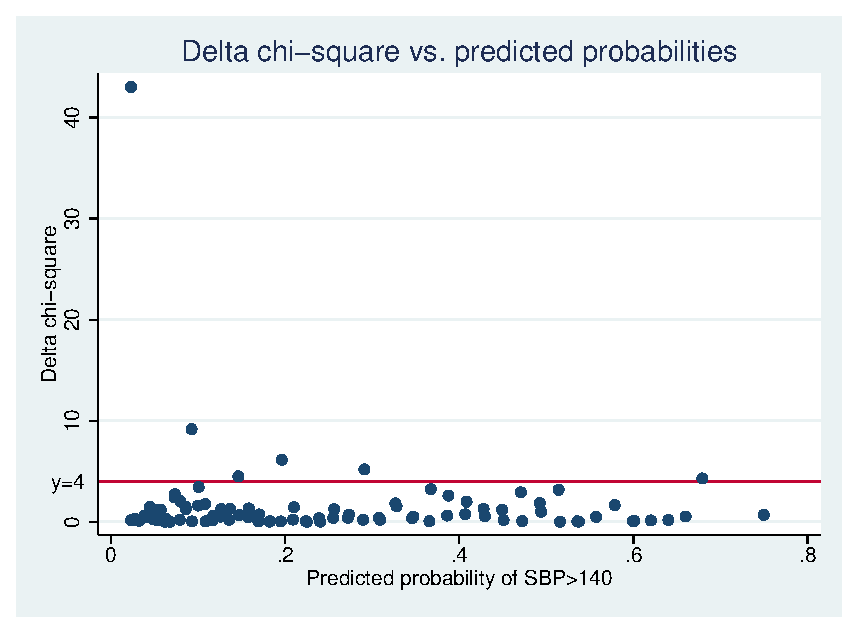
\includegraphics[width=\figwidths]{04/part4_Deltachisq_p_.eps}
    \end{figure} 
    
    \begin{figure}
    \centering
    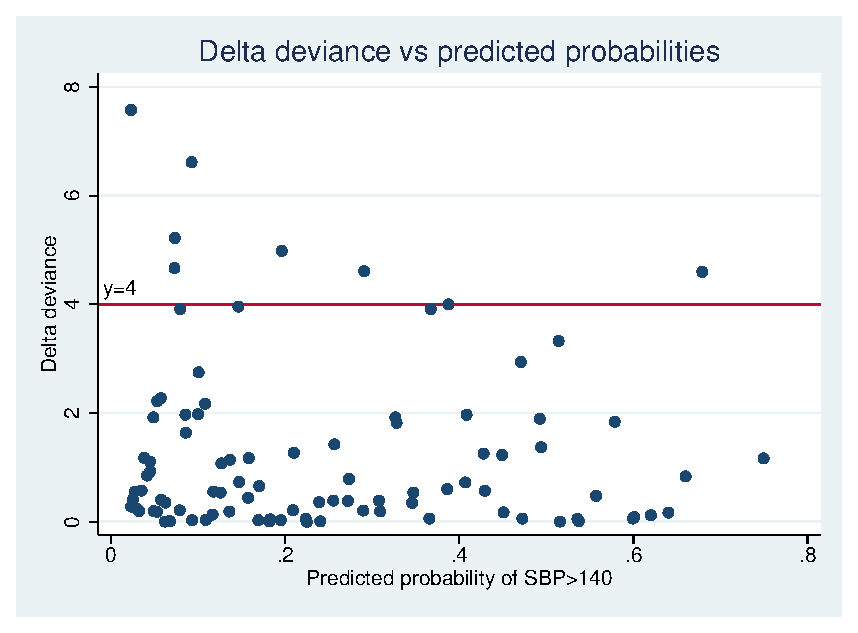
\includegraphics[width=\figwidths]{04/part4_Deltadevi_p_.eps}
    \end{figure} 
    
    \begin{figure}
    \centering
    \includegraphics[width=\figwidths]{04/part4_Deltabeta_p_.eps}
    \end{figure} 

    \begin{figure}
    \centering
    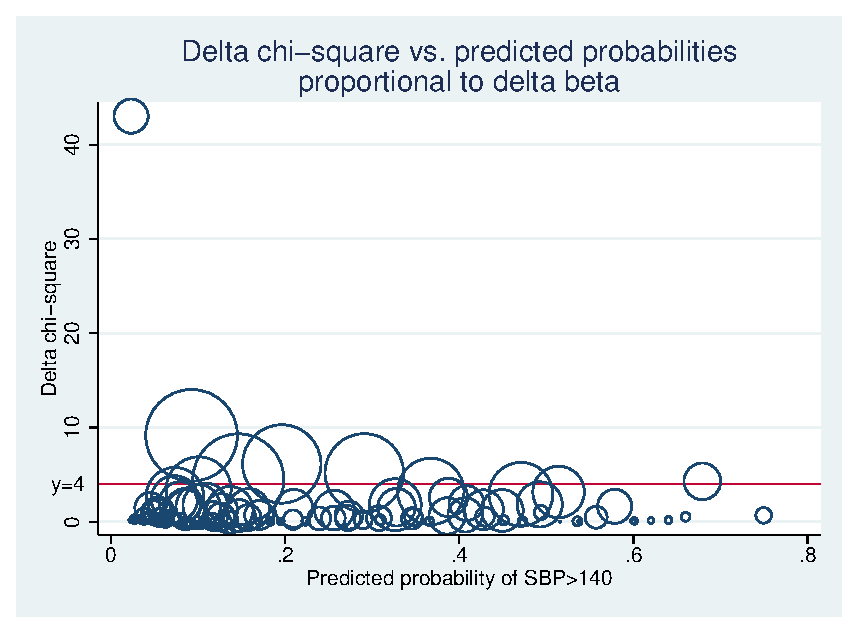
\includegraphics[width=\figwidths]{04/part4_Deltachisq_p_beta_.eps}
    \end{figure}

% This will make the page to avoid mixing figures and code
\pagebreak

      STATA code for 4 plots
      \begin{verbatim}
* plot 1
scatter delta_x2 p, title("Delta chi-square vs. predicted probabilities") ///
    ytitle("Delta chi-square") xtitle("Predicted probability of SBP>140") ///
    yline(4) ttext(4 -0.05 "y=4")
graph export part4_Deltachisq_p_.eps, replace

* plot 2
scatter delta_dev p, title("Delta deviance vs predicted probabilities") ///
    ytitle("Delta deviance") xtitle("Predicted probability of SBP>140") ///
    yline(4) ttext(4.3 0.01 "y=4")
graph export part4_Deltadevi_p_.eps, replace

* plot 3 
scatter dbeta p, title("Delta beta vs predicted probabilities") ///
    ytitle("Delta beta") xtitle("Predicted probability of SBP>140") ///
    yline(1) ttext(4.3 0.01 "y=1.0")
graph export part4_Deltabeta_p_.eps, replace

* plot 4
scatter delta_x2 p [w = dbeta], msymbol(circle_hollow) ///
    title("Delta chi-square vs. predicted probabilities" "proportional to delta beta") ///
    ytitle("Delta chi-square") xtitle("Predicted probability of SBP>140") ///
    yline(4) ttext(4 -0.05 "y=4")
graph export part4_Deltachisq_p_beta_.eps, replace


. table age overweight if delta_x2>=4, contents(freq)

----------------------------
          |    overweight   
      AGE |  BMI<25  BMI>=25
----------+-----------------
       32 |                1
       49 |               33
       55 |               79
       67 |      16         
       73 |      12         
       84 |                2
----------------------------

. 
end of do-file

. table age overweight if delta_dev>=4, contents(freq)

----------------------------
          |    overweight   
      AGE |  BMI<25  BMI>=25
----------+-----------------
       32 |                1
       46 |               30
       49 |               33
       54 |      33         
       67 |      16         
       73 |      12         
       84 |                2
----------------------------

. 
end of do-file


    \end{verbatim}
      
      
      \item If you did find possibly problematic observations, describe what your next steps in model fitting might be.
      
      \textit{Solution}: First step is to extract all patients information from the model with possible problematic covariates pattern, and confirm if there are any data entry problem. Next, we can do sensitivity analysis excluding patients with each covariate pattern, and compare beta term, goodness of fit, Hosmer Lemeshow goodness of fit with original model. If we have similar results as before, we gain more confidence on reporting the results we find. It's also possible that we need to add in other covariates, or interaction term to have a better model fit.
      
  \end{enumerate}

\end{document}